\chapter{Rocket science} \label{cha:Rocket-science}

\section{Orbits} \label{sec:Orbits}

A large amount of specialised terminology is used throughout this thesis. It is assumed that professionals within the space industry are already familiar with this terminology, but for the purposes of completeness a quick explanation is provided here. 

Firstly, the motion of bodies in space is defined by their position relative to each other and their velocity relative to each other. These determine their relative orbital energy, $\epsilon$, as shown in equation \eqref{eq:Specific-orbital-energy}, %Note that relative kinetic energy, $\epsilon_k$, is non-negative, but that relative potential energy, $\epsilon_p$, is always negative.
\begin{subequations} \label{eq:Specific-orbital-energy}
\begin{align} 
\epsilon &= \epsilon_k + \epsilon_p \\
&= \frac{v^2}{2} - \frac{\mu}{r}
\end{align}
\end{subequations}
where $\mu$ is the gravitational parameter of the other body.

In the absence of external forces, orbital energy must be conserved. Under this constraint, two-body orbits take the form of conic sections, a mathematical construct studied as early as 200~BC by Apollonius of Perga. The non-degenerate forms of conic sections are a circle, an ellipse, a parabola, and a hyperbola (the degenerate forms are a single point, a straight line, or two intersecting straight lines). Each of these correspond to a particular type of orbit. 

Only two of these conic sections are important. In a frame centred on one of the bodies, a hyperbola describes the path of a second body with net positive orbital energy, and an ellipse describes the path of a second body with net negative orbital energy. A parabola is a special case where relative orbital energy is exactly zero, and a circular orbit is a special case of the ellipse. 

The primary body is at a point mathematically defined by the conic section, called a focus. A number of other parameters are defined for all conic sections, but only shown for an ellipse in \autoref{fig:ellipse} because ellipses are conceptually easier and the majority of \BW's orbit is expected to be elliptical.

\begin{figure} 
\caption{Elliptical parameters.} \label{fig:ellipse}
\centering
\def\svgwidth{0.6\textwidth}
\input{Images/ellipse.pdf_tex}
%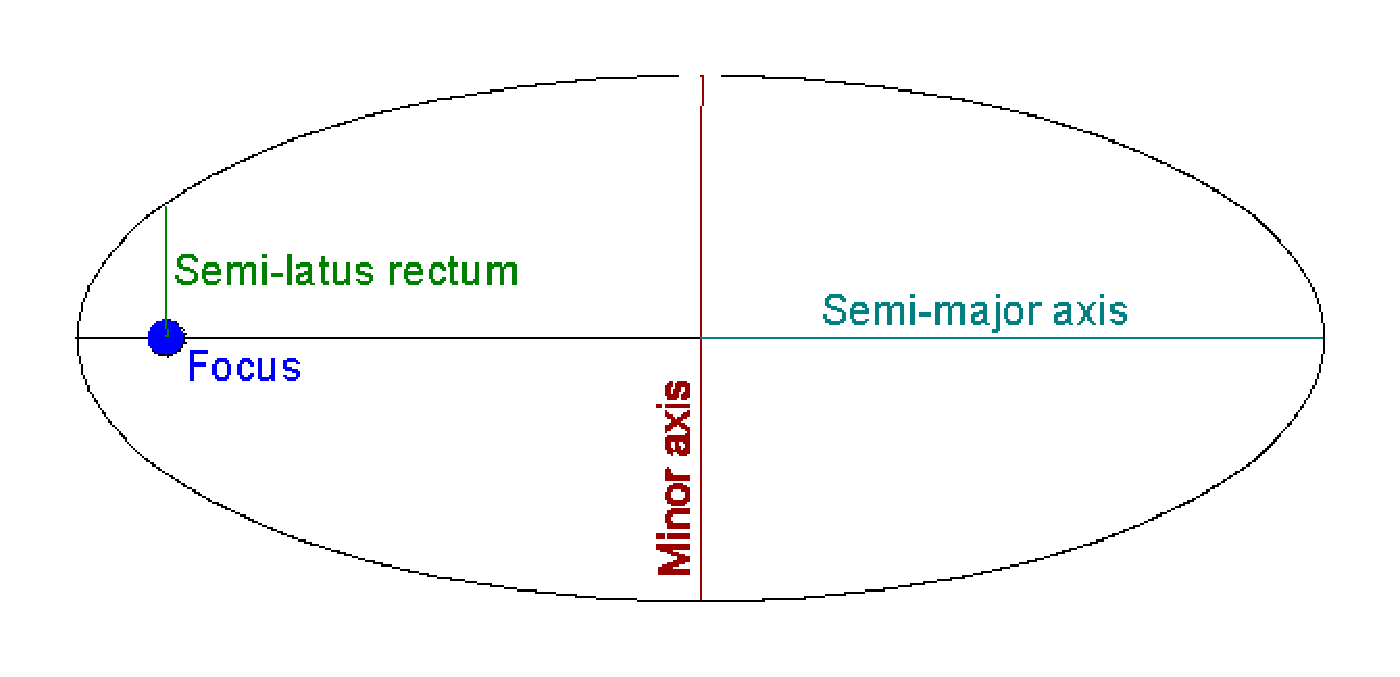
\includegraphics[width=\textwidth]{Images/ellipse_parameters.pdf}
\end{figure}

The semimajor axis, $a$, is half of the length of the major axis, and the semilatus rectum, $p$, is half of the length of the latus rectum. Finally, the \emph{periapsis} is the point in the orbit closest to the primary body, whilst the \emph{apoapsis} is the point furthest from the primary body.


\section{The space environment} \label{sec:Environment}

During the transfer from Earth to Moon, there are a number of issues to consider that may impact the durability of the spacecraft.

\subsection{Van Allen belts} \label{sub:VABs}

The most hazardous element of the journey is radiation. In particular, the Earth's magnetosphere traps particle radiation in two bands above the equator, as seen in the conceptual cross-section in \autoref{fig:vabs}. 

\begin{figure}
\caption{The van Allen Belts conceptual image.} \label{fig:vabs}
\centering
\def\svgwidth{\figurewidth}
\input{Images/vab.pdf_tex}
%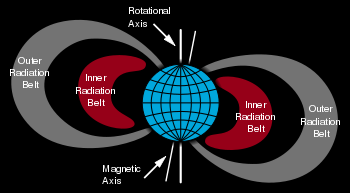
\includegraphics[width=\textwidth]{Images/350px-Van_Allen_radiation_belt_svg.png}
\end{figure}

The outer radiation belt extends from an altitude of about three to ten Earth radii, and is characterised by a relatively high density of high energy (0.1-10~MeV) electrons. The density varies wildly based on geomagnetic storms and variations in solar wind, but an averaged distribution is shown in \autoref{fig:vabs2}.

%\begin{figure} 
%\caption{The AP8MIN van Allen Belt proton flux distribution \parencite{Sawyer1976}. Contours represent particles per square centimetre per second.} \label{fig:vabs2}
%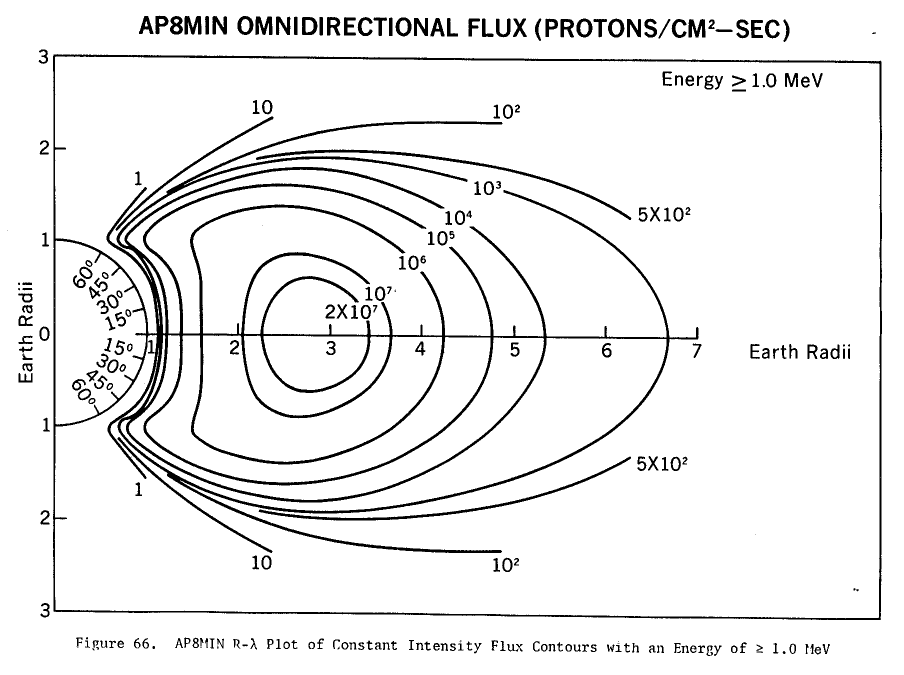
\includegraphics[width=\textwidth,clip,trim=0 35 0 35]{Images/800px-Ap8-omni-1_000MeV.png}
%\end{figure}

\begin{figure} 
\caption{The AP8MIN van Allen Belt proton flux distribution \parencite{Sawyer1976}. Contours represent particles per square centimetre per second.} \label{fig:vabs2}
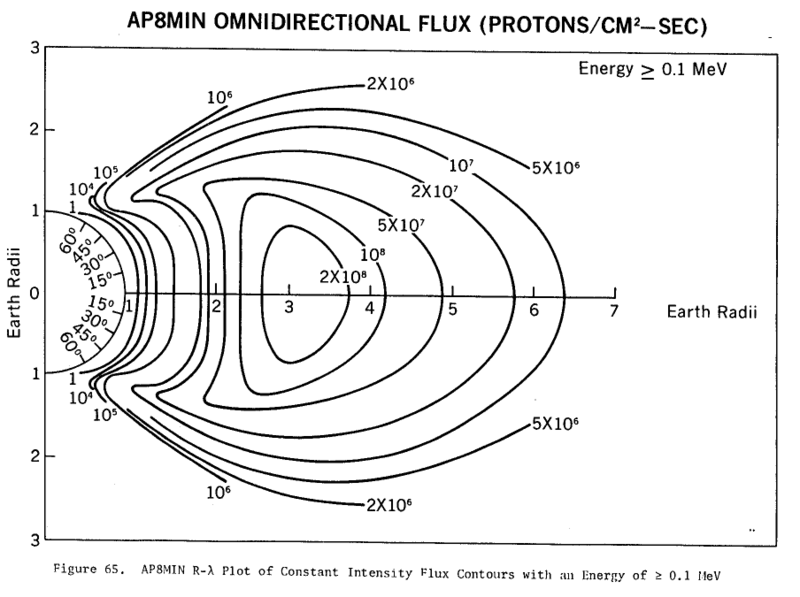
\includegraphics[width=\textwidth,clip,trim=0 35 0 30]{Images/800px-Ap8-omni-0_100MeV.png}
\end{figure}

Much more problematic is the inner belt which extends from an altitude of 100~km (the limit of our atmosphere) to about 10,000~km, and consists of high concentrations of energetic protons (some over 400~MeV, which can penetrate 143~mm of lead) thought to be caused by cosmic ray collisions with nuclei of the upper atmosphere \parencite{Hess1968}.

\begin{figure} 
\caption{The AP8MIN van Allen Belt proton flux distribution \parencite{Sawyer1976}. Contours represent particles per square centimetre per second.} \label{fig:vabs3}
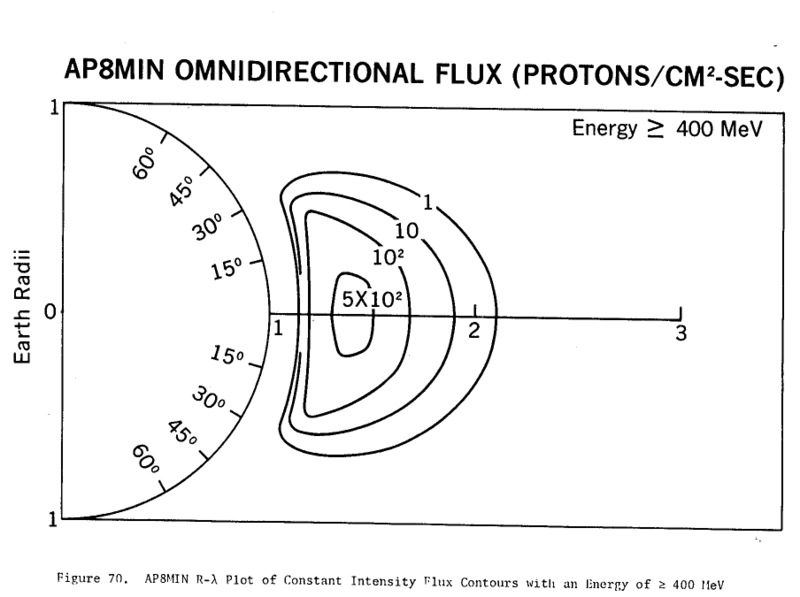
\includegraphics[width=\textwidth,clip,trim=0 35 0 67]{Images/800px-Ap8-omni-400_0MeV.png}
\end{figure}

While the lower energy radiation can and frequently does corrupt computer data on satellites, preventive measures can be taken such as using radiation hardened hardware, or shielding the processors. The higher energy radiation however damages the solar panels, reducing the amount of power they can generate. The only known solution to this problem is to spend as little time within the van Allen belts as possible. This is the reason for the higher thrust ascent phase.

\subsection{Space debris} \label{sub:Debris}

Another hazard to spaceflight is orbital debris, in the form of defunct satellites and rocket parts, as well as micrometeorites. NASA's Orbital Debris Program Office maintains a catalogue of the largest known pieces. Once a completed trajectory is known for \BW, it will be checked against this catalogue. If the trajectory comes within a predetermined safe distance of any known object, it will be recalculated with an adjusted thrust profile or departure date. However, the orbits of smaller pieces of space junk and micrometeorites are unknown, and impacts remain a risk to the mission.

% Figures of merit
\section{Rocket performance}
\subsection{Specific Impulse} \label{sub:Isp}

A key figure in measuring the performance of a thruster is the specific impulse, $I_{sp}$. As mentioned in \autoref{sec:Past-missions}, specific impulse is the momentum added by the thrusters per unit of propellant expended.

Impulse is the scalar sum of force applied over a given time, as shown in equation \eqref{eq:Impulse},
\begin{subequations}
\begin{gather} \label{eq:Impulse}
I = \int_{t_0}^{t_f}\vec{F}\quad dt
\end{gather}
so by \textcite{Newton1687}'s second law $\vec{F} = \frac{d\vec{p}}{dt}$ we get the result in equation \eqref{eq:Impulse2},
\begin{align}\label{eq:Impulse2}
I &= \int_{t_0}^{t_f}\frac{d\vec{p}}{dt}\quad dt \\
&= \int_{t_0}^{t_f}d\vec{p} 
\end{align}
\end{subequations}
which has units of kgms$^{-1}$, and in the special case of collinear forces is equal to the change in momentum $\Delta p$. 

By the conservation of momentum in the satellite's moving frame, the increase in momentum of the spacecraft is equal and opposite to the momentum imparted to the exhaust, as in equation \eqref{eq:Isp},
\begin{subequations}\label{eq:Isp}
\begin{gather}
\Delta p_{craft} - \Delta p_{exhaust} = 0 \\
\Delta p_{craft} = m_{exhaust}v_{exhaust} \\
I = m_{exhaust}v_{exhaust} \\
I_{sp} = v_{exhaust}
\end{gather}
\end{subequations}
so the specific impulse of the spacecraft should be equal to the exhaust velocity, and its units should be ms$^{-1}$. However, the use of imperial units meant that specific impulse was traditionally reported as momentum change per unit {\em weight} of propellant, so the final value is divided by standard gravity on Earth, $g_0$. Consequently specific impulse is reported in seconds.

\begin{equation}
I_{sp}=\frac{v_{ex}}{g_0}
\end{equation}

\subsection{Delta-v} \label{sub:Delta-v}

Since every circular orbit has a unique orbital speed associated with it, a common measure of rocket capability is the change in velocity the rocket can provide. Mathematically, this \emph{delta-v} is calculated as the integral of the acceleration the rocket provides, or more intuitively, the total thrust the rocket provides over time, given by equation \eqref{eq:Delta-V},
\begin{equation}\label{eq:Delta-V}
\Delta v=\int_{t_{0}}^{t_{1}}\frac{T(t)}{m(t)}\quad dt
\end{equation}
where $T(t)$ is the instantaneous thrust magnitude, and $m(t)$ is the instantaneous mass.

Conversely, orbital transfers may be described by the typical change in velocity required. This is known as a delta-v budget. Launching to low Earth orbit (LEO) requires a change of 7.8~kms$^{-1}$, but typically an additional 1.5 to 2~kms$^{-1}$ is lost to atmospheric drag and gravity drag. Ascent from LEO to low lunar orbit (LLO) requires an additional 4.1~kms$^{-1}$ (this mission profile was used by Apollo). Thrust vectoring adds further losses depending upon the angle of thrust. 

These gravitational, atmospheric and thrust vectoring losses can be calculated with similar integrals over the flight, shown in equation \eqref{eq:Delta-Vs},
\begin{subequations} \label{eq:Delta-Vs}
\begin{gather}
\Delta v_{drag}=\int_{t_0}^{t_1}\frac{D(t)}{m(t)}\quad dt \label{eq:drag-penalty} \\
\Delta v_{gravity}=\int_{t_0}^{t_1}g(r)\cdot\sin\gamma\quad dt \label{eq:gravity-penalty} \\
\Delta v_\varepsilon=\int_{t_0}^{t_1}\frac{T(t)}{m(t)}(1-\cos(\alpha-\varepsilon))\quad dt \label{eq:thrust-vectoring-penalty}
\end{gather}
\end{subequations}
where $D(t)$ is the instantaneous aerodynamic drag magnitude, $g(r)$ is the local gravitational acceleration $r$ metres from the centre of the Earth, $\gamma$ is the angle from the velocity vector to the horizontal, $\alpha$ is the body axis line (above the velocity vector) and $\varepsilon$ is the thrust vector (above the body axis line), as shown in \autoref{fig:path-angles} \parencite{Tetlow2003}. Because the thrusters of \BW\ are fixed relative to the body, the thrust vector is fixed at $\varepsilon=0\degrees$.

\begin{figure}
\caption{Flight angle and thrust vector of the spacecraft relative to LVLH frame. $\vec{i}_r$ and $\vec{i}_\theta$ are the local vertical and horizontal, respectively (see \autoref{sec:Reference-frames} for definition). The thrust vector is $\vec{u}$ and the velocity vector is $\vec{v}$. The body axis line represents the orientation of the vehicle.} 
\label{fig:path-angles}
\centering
\def\svgwidth{0.4\textwidth}
\input{Images/flight-angle.pdf_tex}
\end{figure}

Little can be done within the scope of this project to reduce atmospheric drag and gravity drag, since these effects are strongest during launch. However, gravity drag is still present during orbit raising if the thrust line has any component parallel to the gravitational force; when this occurs, the thrust is fighting against gravity rather than increasing the velocity of the spacecraft (and providing delta-v). Similarly, thrust vectoring decreases effective delta-v because the thrust is changing the direction of the spacecraft, rather than increasing its speed. 
% These parameters will be monitored throughout the optimisation, and if gravity drag is significant modifications will be made to improve the results, for example by relaxing the constraints on thrust angle.
 
Delta-v forms a very important performance criterion. It is particularly important in tracking gravitational assists from the Moon, as velocity may be gained without expending delta-v in the form of thrust. Initial simulations at the Institut f\"{u}r Raumfahrtsystem determined an approximate benchmark of 3.5~kms$^{-1}$ for \BW\ \parencite{Roeser2006}. This includes an estimated 1.1~kms$^{-1}$ in phase 2 to ascend beyond the van Allen belts, 1.6~kms$^{-1}$ in phase 3 to cruise to near EML1, 0.5~kms$^{-1}$ in phase 4 to be captured into a lunar orbit, and 0.4~kms$^{-1}$ in phase 5 to descend into the operating orbit.

\subsection{Tsiolkovsky's rocket equation} \label{sec:Tsiolkovsky}

A well established equation, derived in the 19th century by Konstantin Tsiolkovsky and shown in \eqref{eq:Tsiolkovsky}, describes the delta-v available from expending a given mass of fuel from the vehicle at a given exhaust velocity,
\begin{equation}\label{eq:Tsiolkovsky}
\Delta v=v_{e}\ln\frac{m_{0}}{m_{1}}
\end{equation}
where $m_{0}$ represents the initial wet mass of the rocket (structural mass plus fuel), $m_{1}$ represents the final mass, $v_{e}$ is the effective exhaust velocity \parencite{Tsiolkovsky1903,Chobotov2002}. Tsiolkovsky's rocket equation \eqref{eq:Tsiolkovsky} is particularly relevant to low thrust missions because it shows that the most efficient way to achieve a fixed delta-v requirement such as an Earth escape orbit or lunar transfer orbit, is to increase the propellant exhaust velocity. Missions such as \BW\ maximise their delta-v by increasing propellant exhaust velocity at the expense of other design parameters, such as thrust.

The SIMPLEX pulsed plasma thrusters developed at the Institut f\"{u}r Raumfahrtsysteme \parencite{Nawaz2008} provide an exhaust velocity of about 27000~ms$^{-1}$ as stated in \autoref{tab:BW1-performance}, resulting in a specific impulse of about 2750~s. Assuming a dry mass of 150~kg, 75~kg of fuel should allow for a delta-v of 10.9~kms$^{-1}$, far more than is theoretically required for ascent from GTO to lunar orbit.

% \begin{equation}
% \Delta v= c_{PPT}\ln\frac{m_4}{m_3}+c_{arcjet}\ln\frac{m_3}{m_2}+c_{PPT}\ln\frac{m_2}{m_1}+c_{arcjet}\ln\frac{m_1}{m_0}
% \end{equation}



\section{Sphere of influence} \label{sec:SOI}
The sphere of influence approximates the region of space in which a primary body dominates the gravitational forces on any small object such as a spacecraft. This is traditionally used to determine coasting trajectories of chemically propelled spacecraft, thus ignoring third-body gravitational forces. Due to the longer transfer times of low-thrust spacecraft it is necessary to include these additional gravitational forces across the entire trajectory, although the sphere of influence provides a convenient point to switch reference frames. The sphere of influence is defined in equation \eqref{eq:SOI},
\begin{equation}
r_{SOI}=a_{s}\left(\frac{m_{p}}{m_{s}}\right)^{\frac{2}{5}} \label{eq:SOI}
\end{equation}
where $m_{p}$ and $m_{s}$ are the mass of the primary and secondary bodies, respectively, and $a_{s}$ is the semimajor axis of the secondary body's orbit around the primary \parencite{Kemble2006}. The Earth-Moon system spheres of influence are as shown in \autoref{fig:Spheres-of-Influence}.
 Note that the Moon's sphere of influence (with respect to the Earth)\footnote{calculated as just over 66,000~km from the Moon's centre, just under 5/6 of the distance from the Earth to the Moon.} lies entirely within the Earth's (with respect to the Sun)\footnote{calculated as almost 925,000~km from the Earth's centre.}.

\begin{figure} [h]
\caption{Earth and Moon spheres of influence.} \label{fig:Spheres-of-Influence}
\centering
\def\svgwidth{\figurewidth}
\input{Images/soi.pdf_tex}
%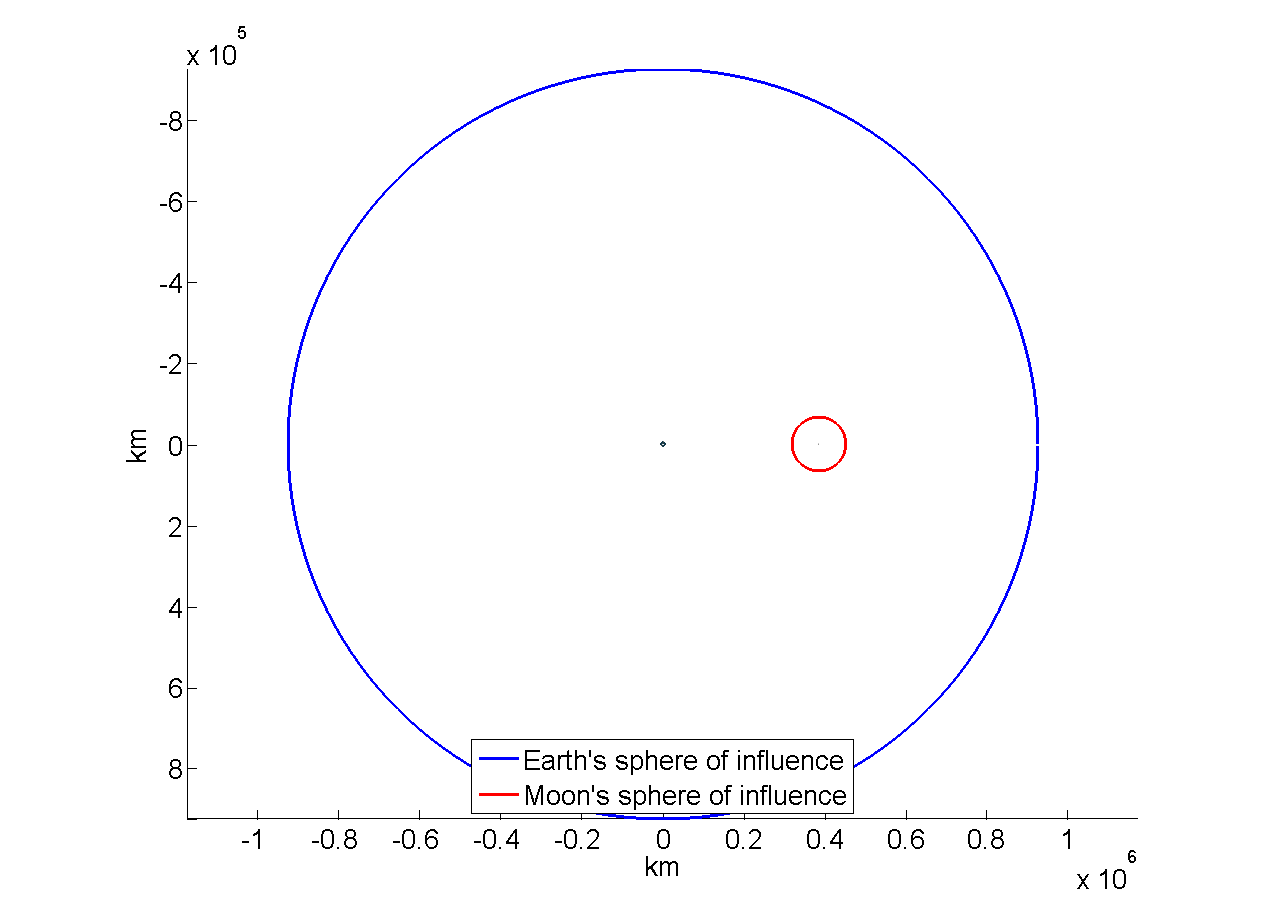
\includegraphics[scale=0.4]{Images/Spheres-of-Influence.png}
\end{figure}

\section{Summary} \label{sec:Rocket-science-summary}

A number of important phenomena related to the lunar trajectory were presented in this section. First, terminology related to elliptical and hyperbolic orbits was introduced for later sections. Then hazards to the mission were presented, notably the radiation in the van Allen belts and space debris. A number of performance measures were then outlined, before the sphere of influence was defined.
